
\documentclass[a4paper,12pt,twocolumn]{article}
\usepackage{geometry}
\usepackage{fontspec}
\usepackage{xeCJK}
\usepackage{graphicx}
\usepackage{array}
\usepackage{booktabs}
\usepackage{longtable}
\usepackage{hyperref}
\usepackage{caption}
\usepackage{indentfirst}
\geometry{left=1.5cm,right=1.5cm,top=1.7cm,bottom=1.8cm,columnsep=0.75cm}
\setmainfont{Times New Roman}
\setCJKmainfont{PMingLiU}
\XeTeXlinebreaklocale "zh"
\XeTeXlinebreakskip = 0pt plus 1pt
\hypersetup{colorlinks=true, linkcolor=black, urlcolor=blue, citecolor=black}
\setlength{\parindent}{2em}
\setlength{\parskip}{0.3em}
\captionsetup{font=small}

\begin{document}

\begin{center}
{\LARGE \textbf{EMCAD 論文閱讀、方法理解與復現報告}}\\[0.4em]
{\large EMCAD: Efficient Multi-scale Convolutional Attention Decoding for Medical Image Segmentation}\\[0.5em]
姓名：丁聖懿 \quad
學號：412770256
\end{center}

\textbf{關鍵字：} 醫學影像分割、解碼器設計、多尺度卷積、注意力機制、復現實驗

\section*{一、簡介}
醫學影像分割的目標，是讓模型把器官、病灶或其他重要區域從影像中準確找出來。這件事看起來像一般的影像分割，但實際上更難，因為醫學影像常常有三個問題：第一，目標大小差很多，小病灶可能只佔畫面很小一塊，大器官卻可能占掉大半張圖；第二，邊界不一定清楚，尤其是內視鏡或超音波影像，常常有模糊、反光或雜訊；第三，資料量比一般自然影像少，模型如果太大，很容易出現訓練成本高、部署困難，甚至過度依賴硬體的情況。

近年很多方法把重點放在 encoder，也就是負責「看圖、抽特徵」的前半段，例如 CNN 或 Transformer。可是作者認為，decoder，也就是把多層特徵慢慢還原成分割圖的後半段，也同樣關鍵。如果 decoder 太簡單，深層特徵和淺層特徵沒有融合好，邊界會不準；如果 decoder 太重，又會讓參數量和計算量大幅增加，不利於實務應用。EMCAD 這篇論文的核心想法，就是不要一味把模型做大，而是重新設計 decoder，讓它在保留多尺度資訊的同時，還能維持較低的計算成本。

本文主要分成兩個部分。前半段整理 EMCAD 想解決的問題，以及作者提出的方法為什麼有效；後半段則根據官方程式碼與這次實驗條件，說明 ClinicDB 與 Synapse 兩個資料集的復現結果。前者屬於二元分割，適合檢查模型是否能穩定回到論文數字；後者屬於多器官分割，任務難度更高，也更能看出模型在複雜情境下的表現。整體內容以論文方法理解、實驗設定與實際復現情況為主。另外，這次整理後的程式、報告與主要實驗結果，也已放在 GitHub 倉庫：\url{https://github.com/a2215489149/EMCAD_Reproduction}。

\section*{二、提出方法}
\subsection*{2.1 作者想解決的問題}
作者觀察到，許多分割模型的 encoder 已經很強，但 decoder 常有兩種問題。第一種是太重，像是大量堆疊標準卷積或複雜跳接融合，雖然效果不錯，但參數和 FLOPs 都很高。第二種是太單純，只做上採樣再相加，雖然速度快，卻不一定能把不同尺度的資訊整理好。醫學影像裡常常同時存在大範圍器官和小區域細節，如果 decoder 只看到單一尺度，很容易出現「大形狀對了，但邊界模糊」或「小目標直接漏掉」的情況。

所以，這篇論文的出發點很明確：作者不是想再做一個更大的 backbone，而是想設計一個更有效率的 decoder，讓模型在不大幅增加硬體成本的前提下，仍然能把不同尺度的特徵收集回來，並且把重要區域與邊界修整得更好。換句話說，EMCAD 想回答的問題是：「能不能用更省的 decoder，做到比現有 decoder 更好的分割效果？」

\subsection*{2.2 EMCAD 的整體概念}
EMCAD 並沒有把整個分割流程完全推翻。它仍然使用 PVTv2 這種 Transformer encoder 先抽出多層特徵，再把這些特徵送進 decoder。真正改動最大的地方，是作者把 decoder 做成一個逐層細化的結構。比較直白地說，encoder 前面已經幫模型看到了不同解析度的內容，而 EMCAD 要做的事情，就是在往上還原影像的過程中，讓這些特徵可以用更省計算量的方式互相補強，而不是只是「拉大尺寸」而已。

如果把它想像成一個學生在畫器官輪廓，encoder 像是在遠處先看出大概位置，decoder 則是在靠近後慢慢補細節。EMCAD 的設計重點，就是讓這個「補細節」的過程不會太昂貴，同時又能確實看到大範圍與小範圍資訊。作者把這件事情拆成幾個模組來做，包含多尺度卷積、注意力篩選、有效率的上採樣，還有多階段監督。

\subsection*{2.3 這篇論文的四個關鍵模組}
\subsubsection*{(1) 多尺度深度卷積模組 MSCAM / MSDC}
這是 EMCAD 最重要的設計。作者不用傳統較重的標準卷積，而是採用 depth-wise convolution，也就是把每個通道先分開處理的卷積方式。這樣做的好處是便宜很多。更重要的是，作者不是只放一個卷積核，而是同時使用多種尺度的 kernel。根據論文 Table 5，在 ClinicDB 和 Synapse 上，[1, 3, 5] 這組 kernel 的效果最好，因此作者最後把它當成正式設定。這個設計的直覺很好理解：1x1 比較像做通道內的重新整理，3x3 可以抓局部形狀，5x5 可以看稍微大一些的範圍，三者一起用，比只看單一尺度更合理。

\subsubsection*{(2) LGAG}
論文中的 LGAG 全名是 large-kernel grouped attention gate，可以把它理解成「在跳接特徵送回 decoder 之前，先過濾一次」。這一點很重要，因為 encoder 早期層的特徵雖然解析度高，但裡面也常有背景雜訊。如果每一層特徵都直接加回 decoder，模型有時反而會被不重要的訊息干擾。LGAG 的作用，就是幫模型先看一下哪些區域比較值得保留，哪些部分可以弱化，讓跳接特徵更像「有挑過的提示」，而不是整包原封不動地送回來。

\subsubsection*{(3) EUCB}
這個模組可以看成比較有效率的上採樣區塊。一般 decoder 一路往上恢復解析度時，如果每一步都用較重的運算，整體成本會很快膨脹。EUCB 的目的，就是把上採樣做得更輕，同時維持足夠的表達能力。這個設計搭配前面的多尺度卷積，形成一種很實際的平衡：該補資訊的地方補資訊，該省運算的地方省運算。

\subsubsection*{(4) 多階段監督}
EMCAD 不是只看最後輸出的分割圖，而是讓 decoder 中間幾層也一起受到監督。實際上這很像老師不只看期末成績，也看幾次平時作業。這種做法通常能讓中間特徵學得比較穩，不會只有最後一層在硬撐。官方程式中對應的是多輸出監督與 MUTATION loss 的設定。即使讀者不去深究每個 loss 名稱，也可以先抓住它最重要的意思：作者希望整個 decoder 的每一步都朝正確方向修正，而不是等到最後一張圖才一次算總帳。

\subsection*{2.4 為什麼這些設計有效}
如果只看論文文字，EMCAD 可能會讓人覺得只是「把很多模組堆在一起」。但作者其實有做相對清楚的驗證。以 Synapse 為例，Table 4 顯示當模型從最基本架構一路加入 cascaded 結構、LGAG、MSCAM 後，平均 Dice 從 80.10 提升到 83.63。這代表這幾個模組不是裝飾，而是真的有在改善結果。再看 Table 6，作者拿 EMCAD 和前一代 CASCADE decoder 比較，在 PVTv2-B2 encoder 上，EMCAD 不只平均 Dice 從 82.78 提升到 83.63，decoder FLOPs 還從 1.93G 降到 0.381G，參數量從 9.27M 降到 1.91M。這組數字非常有說服力，因為它證明作者不是只追求高分，而是同時做到「更輕」與「更好」。

從讀者角度來看，EMCAD 的重點貢獻可以整理成一句話：作者把 decoder 這個常常被當成配角的部分重新做好，讓模型在多尺度理解、跳接特徵過濾、以及運算效率三件事情之間取得更好的平衡。這也是為什麼 EMCAD 不是只在單一資料集有效，而是能在多種 2D 醫學影像分割任務上都拿到不錯結果。

\section*{三、實驗設計與復現結果}
\subsection*{3.1 論文設定與這次實驗條件}
根據原論文 Section 4.1，作者使用單張 NVIDIA RTX A6000 48GB 搭配 PyTorch 1.11.0 來訓練模型，前端特徵抽取採用 ImageNet 預訓練的 PVTv2-B0 或 PVTv2-B2，參數更新方式使用 AdamW。學習率和權重衰減都設為 1e-4。大多數只有前景與背景兩類的資料集都訓練 200 個 epochs，每次送入 16 張影像；但 Synapse 例外，需要訓練 300 個 epochs，每次送入 6 張影像，輸入大小為 224x224，損失函數則是交叉熵和 Dice 的加權組合。ClinicDB 這類資料則使用 352x352 影像，並配合多尺度訓練。論文表格中的 EMCAD 成績，原則上都是五次實驗的平均值。

本次復現在個人電腦環境中進行，主要硬體是 RTX 4070 SUPER 12GB。軟體版本則盡量貼近作者設定，使用 Python 3.8 與 PyTorch 1.11.0+cu113。因為顯示卡記憶體比論文使用的 A6000 小很多，所以 ClinicDB 每次送入的張數改成 8，Synapse 維持 6。這種調整只是配合機器條件，沒有去改模型本身。文中使用的數據，都是根據官方程式、官方測試流程和當時保留下來的模型權重整理而成。

\begin{table*}[t]
\centering
\caption{原論文設定與這次復現設定比較}
\scriptsize
\setlength{\tabcolsep}{5pt}
\renewcommand{\arraystretch}{1.18}
\begin{tabular}{l l l}
\toprule
\textbf{項目} & \textbf{原論文} & \textbf{這次復現} \\
\midrule
硬體 & NVIDIA RTX A6000 48GB & RTX 4070 SUPER 12GB \\
框架 & PyTorch 1.11.0 & PyTorch 1.11.0+cu113 \\
Encoder & PVTv2-B0 / PVTv2-B2 & PVTv2-B2 \\
ClinicDB & 200 epochs, bs 16, 352x352, 5 runs & 200 epochs, bs 8, 352x352, 先完成有效的第 1 次實驗 \\
Synapse & 300 epochs, bs 6, 224x224, 5 runs & 最佳結果在第 60 個 epoch，訓練持續到第 75 個 epoch \\
驗收方式 & 以五次平均報告 & 先檢查是否接近論文，再說明是否完成完整訓練流程 \\
\bottomrule
\end{tabular}
\end{table*}

Table 1 顯示，這次復現和原論文最大的差別，其實不在方法本身，而在硬體條件。原論文使用 48GB 顯示卡，這次只有 12GB，所以能同時送進模型的影像較少，長時間訓練也比較吃力。也因為這樣，ClinicDB 先拿來確認模型能不能回到論文數字附近；Synapse 則先用目前最好的權重做正式測試，再判斷和論文還差多少。

\subsection*{3.2 ClinicDB：先修正資料問題，再談模型表現}
ClinicDB 一開始的問題不是模型，而是資料本身。照官方連結下載後，實際去看資料夾，發現 train、val、test 每一邊都只有 50 張圖片，這和論文補充資料提到的 612 張影像、80:10:10 的切分明顯對不上。既然訓練資料少了一大截，當時跑出的分數自然不能直接拿來和論文比較。

後來重新排查後可以確認，EMCAD 的訓練程式本身沒有先出問題，真正的原因是資料沒有下載完整。把資料補齊後，ClinicDB 才回到正確規模，也就是 train 489、val 61、test 62。在這種條件下重新跑官方流程，得到的數字才有意義。

\begin{table*}[t]
\centering
\caption{ClinicDB 資料問題修正前後比較}
\scriptsize
\setlength{\tabcolsep}{7pt}
\renewcommand{\arraystretch}{1.18}
\begin{tabular}{l l c c}
\toprule
\textbf{狀態} & \textbf{資料數量} & \textbf{Dice} & \textbf{HD95} \\
\midrule
修正前的不完整資料 & train 50 / val 50 / test 50 & 84.3708 & 27.5559 \\
修正後的正確資料 & train 489 / val 61 / test 62 & 95.2186 & 6.2923 \\
\bottomrule
\end{tabular}
\end{table*}

資料補齊後，ClinicDB 的正式測試結果中，最重要的 Dice 是 95.2186，和論文 Table 1 的 95.21 幾乎一樣，差值只有 +0.0086。其他常見指標像 IoU 91.1235、Sensitivity 95.3200、Specificity 99.7263、Precision 95.4610 和 HD95 6.2923，也都維持在合理範圍。這說明前面只有 84 分左右的結果，主要不是模型太差，而是資料條件一開始就不對。

Table 2 把資料修正前後的差別直接列出來。修正前的 train 50 / val 50 / test 50，並不是論文使用的 612 張影像切分，因此當時算出的分數不能當成有效重現結果。修正後回到 train 489、val 61、test 62，才具備和論文數字比較的前提。

\begin{table*}[t]
\centering
\caption{ClinicDB 相關結果，參考原論文 Table 1 的呈現方式}
\scriptsize
\setlength{\tabcolsep}{8pt}
\renewcommand{\arraystretch}{1.18}
\begin{tabular}{l c c c}
\toprule
\textbf{方法} & \textbf{\#Params} & \textbf{\#FLOPs} & \textbf{ClinicDB Dice} \\
\midrule
DeepLabv3+ & 39.76M & 14.92G & 93.24 \\
PolypPVT & 25.11M & 5.30G & 94.13 \\
PVT-CASCADE & 34.12M & 7.62G & 94.53 \\
PVT-EMCAD-B0 & 3.92M & 0.84G & 94.60 \\
PVT-EMCAD-B2（論文） & 26.76M & 5.60G & 95.21 \\
PVT-EMCAD-B2（這次復現） & 26.76M & 5.60G & 95.2186 \\
\bottomrule
\end{tabular}
\end{table*}

Table 3 把這次結果放回原論文 Table 1 的比較脈絡中。PVT-EMCAD-B2 的 Dice 為 95.2186，和論文 95.21 幾乎重合，差值只有 +0.0086。

不過這裡還是要交代清楚，原論文 Table 1 用的是五次實驗平均；目前資料補齊後，我們先完成的是一個有效的第 1 次實驗，用來確認模型是否真的回到論文水準。若要把整張表完整重建，後面仍要把修正後的資料再多跑幾次，才能算平均值和變動範圍。也就是說，ClinicDB 這裡已經可以說「有重現到」，但還不是完整的五次平均版本。

\subsection*{3.3 Synapse：資料沒有大問題，但完整訓練成本很高}
Synapse 和 ClinicDB 不一樣，主要問題不在資料缺漏。這組資料在檢查後，訓練切片共有 2211 個，測試用的 3D 影像有 12 個，和官方流程大致對得上。所以這一組真正的難點，不是資料有沒有抓錯，而是原論文要求的訓練時間很長，個人電腦能不能撐到同樣的訓練長度。

依照原論文設定，Synapse 要訓練 300 個 epochs，而且表格中的 EMCAD 成績也是五次平均。這在 RTX A6000 48GB 上比較容易完成，但在 RTX 4070 SUPER 12GB 上成本就高很多。從實驗紀錄來看，訓練從第 41 個 epoch 接著跑到第 75 個 epoch，平均一個 epoch 大約要 15.7 分鐘。照這個速度估算，若完整跑到 300 個 epochs，大約需要 78.5 小時，還不包含中途重跑和正式測試的時間。另外，Synapse 的官方正式測試在個人電腦上單次也大約要 35.8 分鐘，所以這不是短時間就能確認完的資料集。

目前最好的模型權重出現在第 60 個 epoch，之後訓練雖然繼續到第 75 個 epoch，但期中階段還沒完整走完 300 個 epochs。中間原因很實際：訓練曾一度中斷，後來才接著跑回去；而當分數已經接近論文時，又先插入一次官方正式測試，確認目前的權重到底到什麼程度。換句話說，這裡不是完全沒做到，而是已經跑到一個接近論文的權重，但還沒把整個論文要求的訓練長度和五次平均全部補完。

\begin{table*}[t]
\centering
\caption{Synapse 相關結果，參考原論文 Table 2 的呈現方式}
\scriptsize
\setlength{\tabcolsep}{9pt}
\renewcommand{\arraystretch}{1.18}
\begin{tabular}{l c c c}
\toprule
\textbf{方法} & \textbf{Avg Dice} & \textbf{HD95} & \textbf{mIoU} \\
\midrule
PVT-CASCADE & 81.06 & 20.23 & 70.88 \\
TransCASCADE & 82.68 & 17.34 & 73.48 \\
PVT-EMCAD-B2（論文） & 83.63 & 15.68 & 74.65 \\
PVT-EMCAD-B2（這次最佳權重） & 81.7860 & 17.8024 & 72.3873 \\
\bottomrule
\end{tabular}
\end{table*}

Synapse 的正式測試結果為平均 Dice 81.7860、HD95 17.8024、mIoU 72.3873，另外平均 ASD 為 3.3085。若只看 Dice，和論文相比差了 -1.8440；HD95 與 mIoU 的差距則分別是 +2.1224 與 -2.2627。以這次期中先用 Dice 相差 2 個百分點內作為接近標準來看，這個權重檔已經算達標；但若依照最嚴格的論文重現標準，它還不能算完整重現，因為 300 個 epochs 和五次平均都還沒做完。

Table 4 把這次最好的權重結果和論文數字並排放在一起。從表中可以看出，Synapse 已經接近論文水準，但還不能說完全對齊，因為目前仍少了完整訓練長度與多次平均這兩個條件。

\begin{table*}[t]
\centering
\caption{復現結果摘要}
\scriptsize
\setlength{\tabcolsep}{7pt}
\renewcommand{\arraystretch}{1.18}
\begin{tabular}{l l c c c}
\toprule
\textbf{資料集} & \textbf{指標} & \textbf{論文數值} & \textbf{這次數值} & \textbf{差值} \\
\midrule
ClinicDB & Dice & 95.21 & 95.2186 & +0.0086 \\
ClinicDB & HD95 & -- & 6.2923 & -- \\
Synapse & Mean Dice & 83.63 & 81.7860 & -1.8440 \\
Synapse & HD95 & 15.68 & 17.8024 & +2.1224 \\
Synapse & mIoU & 74.65 & 72.3873 & -2.2627 \\
\bottomrule
\end{tabular}
\end{table*}

Table 5 把 ClinicDB 與 Synapse 的主要指標集中整理。ClinicDB 使用的是官方測試結果；Synapse 則是用目前最好的權重去做正式測試，因此還不能把它看成完整的 300 個 epochs 與五次平均結果。

\subsection*{3.4 結果整理與限制}
整體來看，ClinicDB 已非常接近論文結果；Synapse 也已經跑到接近論文數字的範圍，但還沒有完成論文要求的完整訓練長度。兩個資料集的差異也很明顯：ClinicDB 的關鍵是資料切分有沒有正確，Synapse 的關鍵則是訓練時間夠不夠、顯示卡撐不撐得住，以及正式測試本身就要花不少時間。

從這次結果來看，EMCAD 在比較有限的硬體條件下，仍然可以維持接近論文的表現，這和論文強調的「用較省的解碼器換到不錯效果」是同一個方向。不過，Synapse 這部分目前仍應視為期中階段結果，而不是完整重現後的最後版本。

\section*{四、結論與討論}
EMCAD 這篇論文的重點，在於作者把設計焦點放在 decoder，而不是只依賴更大的 encoder。整個方法是以 cascaded decoder 為骨架，逐層接收 encoder 傳下來的特徵，再一邊融合、一邊細化分割結果。其中最核心的模組是 MSCAM / MSDC，也就是把 [1, 3, 5] 這組多尺度 depth-wise convolution 放進 decoder，讓模型在還原影像時，同時看到小範圍細節與較大範圍的結構資訊。這個設計能補強醫學影像裡常見的尺度差異問題，例如器官輪廓與細小邊界同時存在時，單一尺度的卷積往往不夠。

除了多尺度卷積之外，EMCAD 也把 skip connection 的處理做得更細。LGAG 先對 encoder 傳回來的特徵做篩選，減少背景雜訊直接混進 decoder；EUCB 則負責較有效率的上採樣，避免 decoder 在恢復解析度時把計算量堆得太高。最後，多階段監督讓中間層的輸出也一起接受訓練訊號，不只看最後一張分割圖。把這幾個模組放在一起後，EMCAD 的方法重點就很清楚了：不是單純追求更大模型，而是希望用更精簡的 decoder，把多尺度資訊、跳接特徵與上採樣流程整理得更有效率。

本次復現的結果可以分成兩部分來看。ClinicDB 在資料修正完成後，官方測試 Dice 為 95.2186，和論文的 95.21 幾乎一致，表示這部分已經回到論文量級。Synapse 方面，目前最佳權重的官方正式測試結果為 Mean Dice 81.7860，和論文的 83.63 仍有差距，但已接近論文結果。這部分的限制主要來自硬體條件、訓練時間，以及尚未完成完整的 300 epochs 與五次平均。

整體而言，這次期中報告已完成論文方法整理與基線驗證。ClinicDB 的結果可作為有效重現紀錄；Synapse 則仍需補足完整訓練與多次實驗，才能和論文表格做更嚴格的對照。這也說明，醫學影像分割的復現不只取決於模型本身，資料條件、訓練設定與硬體環境也都會直接影響最後結果。

\section*{五、改良實驗：ACMS}
\subsection*{5.1 改良想法}
在基線模型能順利重現之後，這次另外做了一個訓練策略上的改良嘗試，名稱為 ACMS。這個做法沒有去改 EMCAD 的網路結構，也沒有增加新的解碼器模組，改動只放在 ClinicDB 的訓練方式。原本的設定會把多個輸出頭相關的監督項目一起打開；ACMS 則把這件事分成兩個階段處理。

第一階段稱為 pool\_a。這個階段只讓四個單獨輸出頭各自學習，目的，是先讓每一層 decoder 的輸出比較穩。第二階段稱為 pool\_b。當相鄰輸出頭之間的差異下降到門檻以下，而且連續維持一段時間後，才把融合後的那一項監督一起打開。這個想法很像先讓每個小組員把自己的部分做好，再要求大家一起交一份整體答案。若太早把融合監督打開，還沒穩定的輸出頭可能會互相干擾。

這次 ACMS 的實驗設定為 threshold 0.22、patience 3、min epoch 15。實際訓練時，模型在第 17 個 epoch 從 pool\_a 切到 pool\_b，代表前面的相鄰輸出頭差異已經連續達到設定門檻。

\subsection*{5.2 實驗圖表與數據}
為了公平比較，這一章使用的 baseline 不是前面用來對論文做正式驗收的那個結果，而是和 ACMS 使用相同資料、相同 batch size、相同 seed 240412 所跑出的對照組。這樣做的目的，是把差異盡量限制在「有沒有開啟 ACMS」這一個變因上。

\begin{table*}[t]
\centering
\caption{ClinicDB 上 baseline 與 ACMS 的比較}
\scriptsize
\setlength{\tabcolsep}{7pt}
\renewcommand{\arraystretch}{1.18}
\begin{tabular}{l c c c c c}
\toprule
\textbf{設定} & \textbf{最佳驗證 Dice} & \textbf{最佳驗證 epoch} & \textbf{對應測試 Dice} & \textbf{測試最高 Dice} & \textbf{和 baseline 比較} \\
\midrule
Baseline & 0.9456 & 114 & 0.9505 & 0.9529 & -- \\
ACMS & 0.9393 & 154 & 0.9502 & 0.9525 & 驗證 -0.0063，測試 -0.0003 \\
\bottomrule
\end{tabular}
\end{table*}

Table 6 顯示，ACMS 跑完 200 個 epochs 後，最佳驗證 Dice 為 0.9393，出現在第 154 個 epoch；在該點對應的測試 Dice 為 0.9502。對照組 baseline 的最佳驗證 Dice 為 0.9456，出現在第 114 個 epoch；該點對應的測試 Dice 為 0.9505。若只看最佳驗證 Dice，ACMS 比 baseline 低了 -0.0063，因此還不能說它已經穩定超過原本方法。

不過，這組結果仍然有觀察價值。這次比較是在相同資料、相同 batch size、相同 seed 下進行，唯一改動只有監督項目切換的時機，因此表中的差異可以比較直接地反映 ACMS 這個想法本身對訓練過程的影響。另一方面，ACMS 的測試集單點最高 Dice 有到 0.9525，baseline 的單點最高則是 0.9529。這表示 ACMS 雖然沒有把主要指標穩定推高，但它並不是完全沒有作用，而是真的改變了模型前後期的學習節奏。

\begin{figure*}[t]
\centering
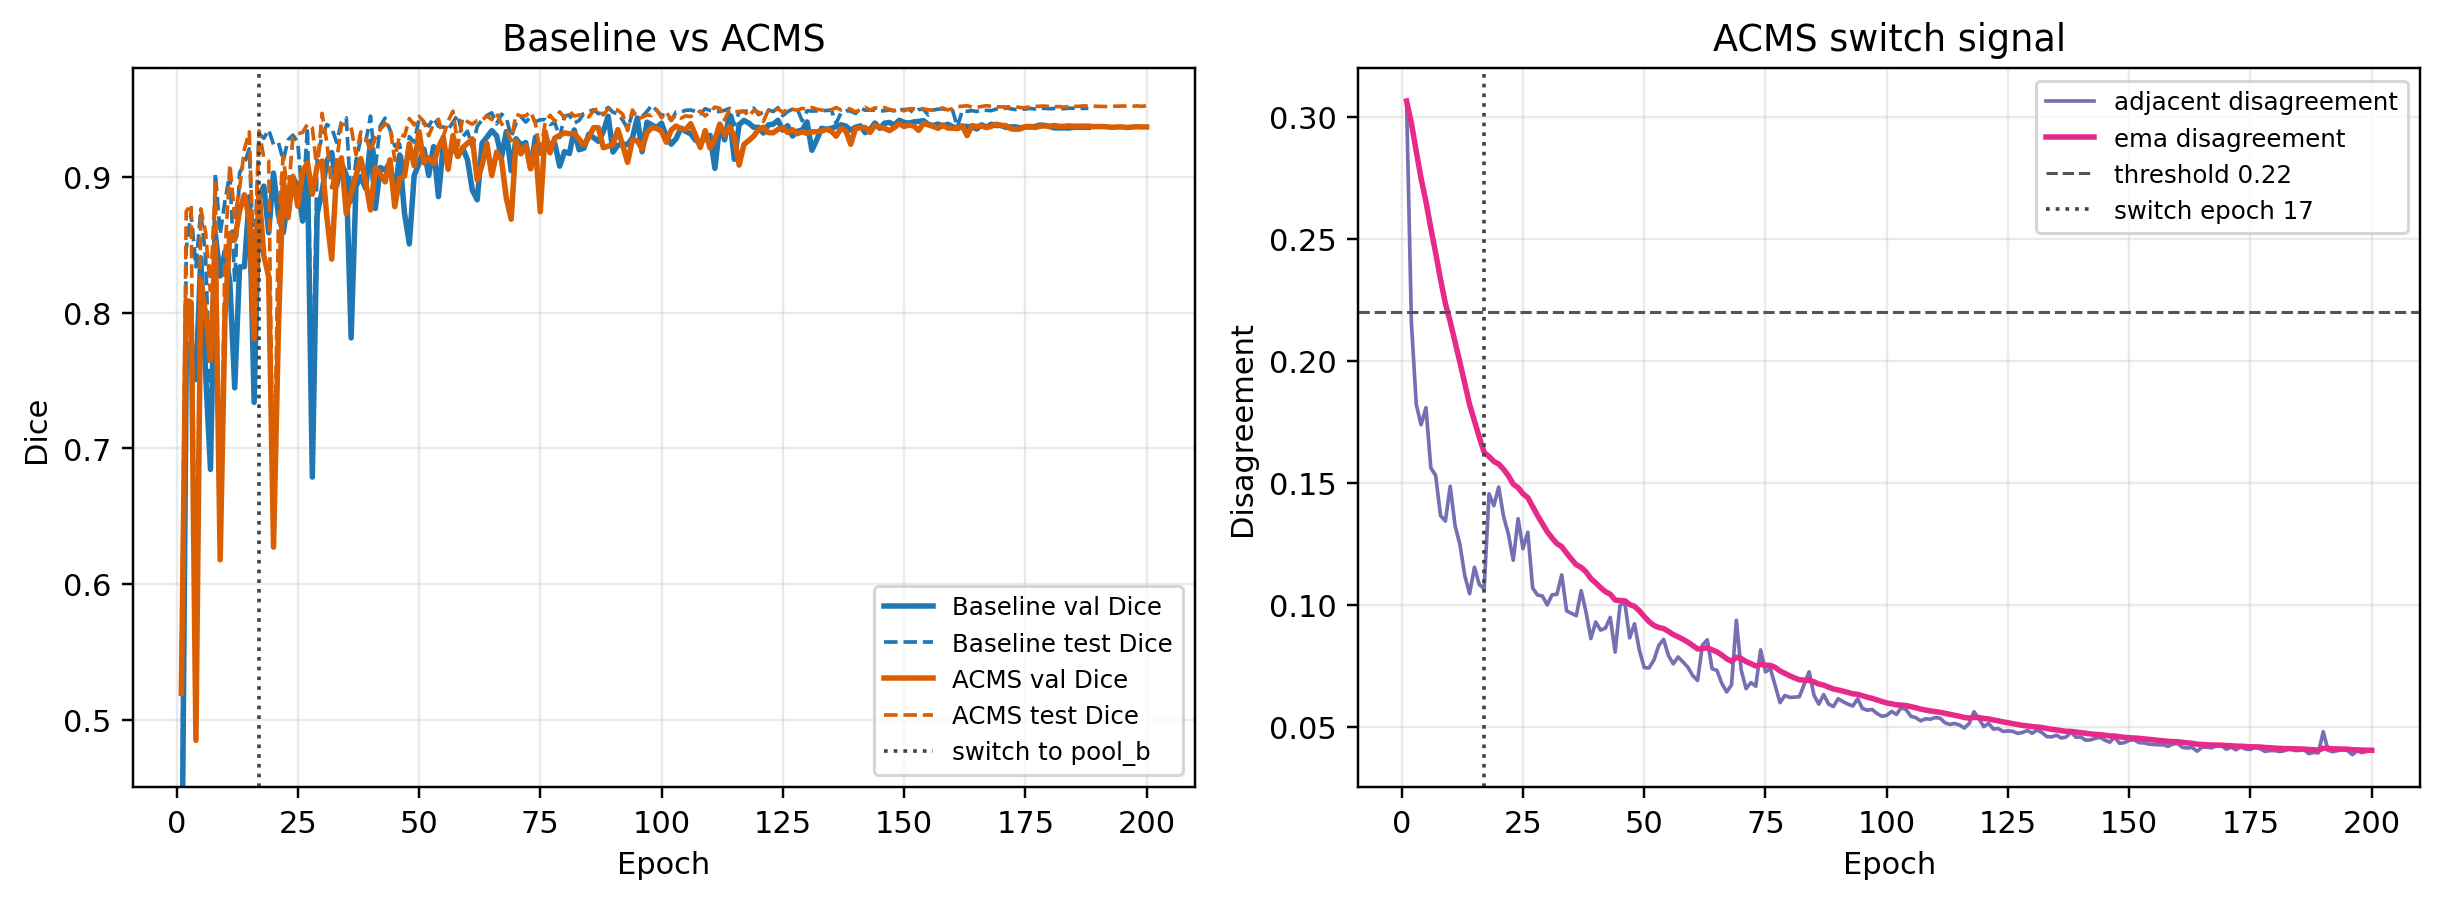
\includegraphics[width=0.96\textwidth]{figures/clinicdb_acms_comparison.png}
\caption{左圖比較 baseline 與 ACMS 在 ClinicDB 上的驗證與測試 Dice 曲線；右圖則顯示 ACMS 用來判斷切換時機的差異值變化。虛線表示切換門檻，垂直線表示從 pool\_a 切到 pool\_b 的位置。}
\end{figure*}

Figure 1 左邊可以看到，ACMS 在前期波動比 baseline 更明顯，但進入後期後仍能回到高分區，沒有出現切換後整體崩掉的情況。右邊則顯示，平滑後的差異值會隨訓練逐漸下降，並在第 17 個 epoch 達到切換條件。這表示 ACMS 不是隨便在某個時間點切換，而是等相鄰輸出頭先接近一致後才進入第二階段。即使最後沒有正式超過 baseline，這個現象本身仍然說明監督時機確實會影響模型的收斂方式。

\subsection*{5.3 結果解讀}
這次 ACMS 的結果，我比較傾向把它看成一次有收穫的嘗試。它現在還不能算改良成功，因為主要指標沒有穩定贏過 baseline；但也不能直接說沒有用，因為整個流程確實有跑完 200 個 epochs。從訓練紀錄來看，pool\_a 到 pool\_b 的切換也有在第 17 個 epoch 正常發生，表示這個兩階段做法至少不是停留在想法。

另外，ACMS 最後還是能收斂到接近 baseline 的區間，這點我覺得也很重要。它代表這個改動沒有把原本 EMCAD 有效的訓練方向帶偏。雖然最佳驗證 Dice 沒有超過 baseline，但部分測試點有追上，甚至短暫更高。這也表示，影響模型表現的不只是網路結構本身，監督項目在什麼時間打開，的確會改變學習過程。

對我來說，這章最有價值的地方，是把後續方向縮小得更清楚。原本如果只說「想改進 EMCAD」，範圍其實太大；做完這次實驗後，至少可以明確知道後面能往切換門檻、切換時機，或不同輸出頭的配重方式繼續調整。也就是說，這次 ACMS 雖然還沒有形成穩定優勢，但它不是白做，而是把下一步該往哪裡改講得更具體。

\clearpage
\section*{參考文獻}
\begin{thebibliography}{99}
\bibitem{emcad}
M. M. Rahman, M. Munir, and R. Marculescu, ``EMCAD: Efficient Multi-scale Convolutional Attention Decoding for Medical Image Segmentation,'' in \textit{Proceedings of the IEEE/CVF Conference on Computer Vision and Pattern Recognition}, 2024.

\bibitem{emcad-supp}
M. M. Rahman, M. Munir, and R. Marculescu, ``Supplementary Material for EMCAD: Efficient Multi-scale Convolutional Attention Decoding for Medical Image Segmentation,'' CVPR 2024.

\bibitem{emcad-repo}
SLDGroup, ``EMCAD official implementation,'' GitHub repository. Available: \url{https://github.com/SLDGroup/EMCAD}

\bibitem{pvtv2}
W. Wang et al., ``PVT v2: Improved Baselines with Pyramid Vision Transformer,'' \textit{Computational Visual Media}, vol. 8, no. 3, pp. 415-424, 2022.

\bibitem{cascade}
M. M. Rahman and R. Marculescu, ``Medical Image Segmentation via Cascaded Attention Decoding,'' in \textit{Proceedings of the IEEE/CVF Winter Conference on Applications of Computer Vision}, 2023.

\bibitem{transunet}
J. Chen et al., ``TransUNet: Transformers Make Strong Encoders for Medical Image Segmentation,'' arXiv:2102.04306, 2021.

\bibitem{polyp-pvt}
D.-P. Fan et al., ``Polyp-PVT: Polyp Segmentation with Pyramid Vision Transformers,'' arXiv:2108.06932, 2021.
\end{thebibliography}

\end{document}
